\documentclass[margin=2mm]{standalone}
\usepackage{tikz}
\usepackage{amsmath,amssymb,mathtools}
\begin{document}
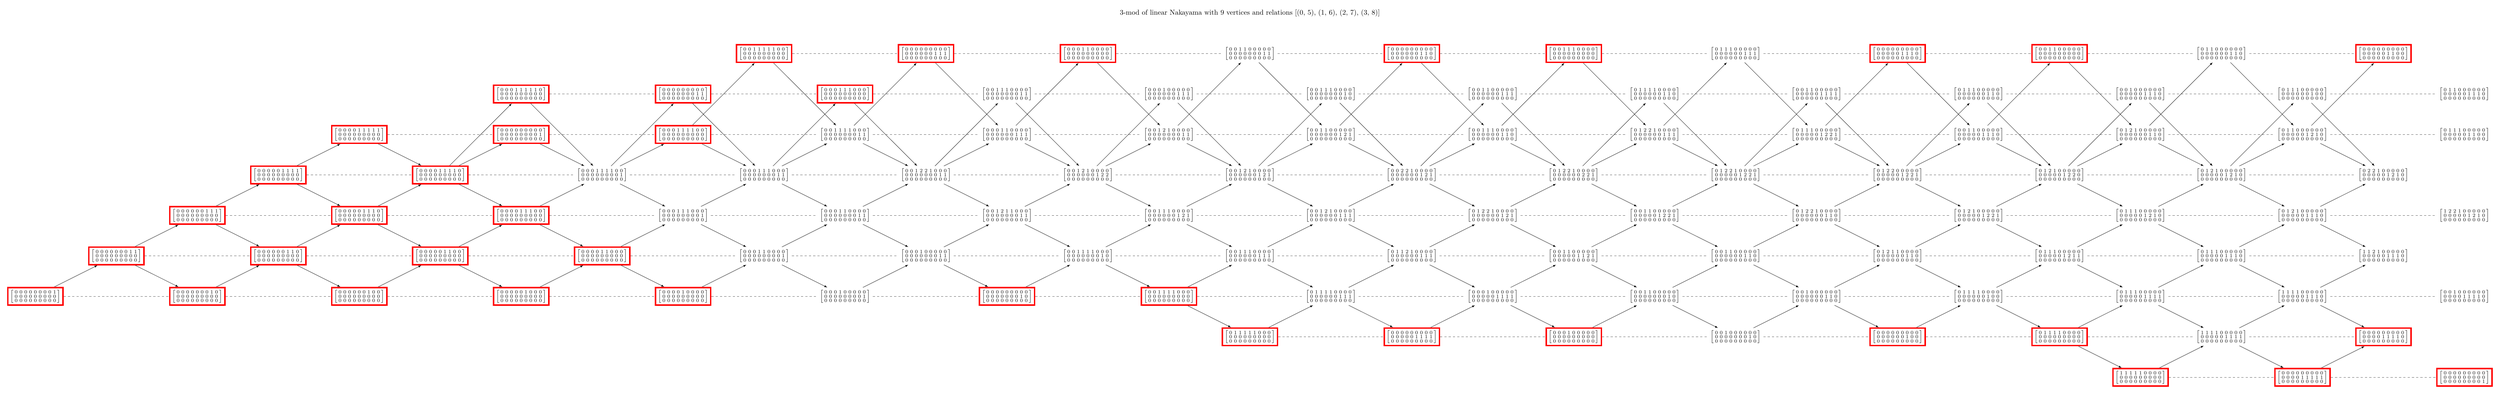
\begin{tikzpicture}[xscale=4,yscale=2]
\node at (15.0,7) [] {$3$-mod of linear Nakayama with 9 vertices and relations [(0, 5), (1, 6), (2, 7), (3, 8)]};
\node (t-0P0) at (26,-2) [scale=1,rectangle,draw=red,line width=2pt] {$\begin{bsmallmatrix}
 1 & 1 & 1 & 1 & 1 & 0 & 0 & 0 & 0\\
 0 & 0 & 0 & 0 & 0 & 0 & 0 & 0 & 0\\
 0 & 0 & 0 & 0 & 0 & 0 & 0 & 0 & 0\\
\end{bsmallmatrix}$};
\node (t-1P0) at (28,-2) [scale=1,rectangle,draw=red,line width=2pt] {$\begin{bsmallmatrix}
 0 & 0 & 0 & 0 & 0 & 0 & 0 & 0 & 0\\
 0 & 0 & 0 & 0 & 1 & 1 & 1 & 1 & 1\\
 0 & 0 & 0 & 0 & 0 & 0 & 0 & 0 & 0\\
\end{bsmallmatrix}$};
\node (t-2P0) at (30,-2) [scale=1,rectangle,draw=red,line width=2pt] {$\begin{bsmallmatrix}
 0 & 0 & 0 & 0 & 0 & 0 & 0 & 0 & 0\\
 0 & 0 & 0 & 0 & 0 & 0 & 0 & 0 & 0\\
 0 & 0 & 0 & 0 & 0 & 0 & 0 & 0 & 1\\
\end{bsmallmatrix}$};
\node (t-0P1) at (15,-1) [scale=1,rectangle,draw=red,line width=2pt] {$\begin{bsmallmatrix}
 0 & 1 & 1 & 1 & 1 & 1 & 0 & 0 & 0\\
 0 & 0 & 0 & 0 & 0 & 0 & 0 & 0 & 0\\
 0 & 0 & 0 & 0 & 0 & 0 & 0 & 0 & 0\\
\end{bsmallmatrix}$};
\node (t-1P1) at (17,-1) [scale=1,rectangle,draw=red,line width=2pt] {$\begin{bsmallmatrix}
 0 & 0 & 0 & 0 & 0 & 0 & 0 & 0 & 0\\
 0 & 0 & 0 & 0 & 0 & 1 & 1 & 1 & 1\\
 0 & 0 & 0 & 0 & 0 & 0 & 0 & 0 & 0\\
\end{bsmallmatrix}$};
\node (t-2P1) at (19,-1) [scale=1,rectangle,draw=red,line width=2pt] {$\begin{bsmallmatrix}
 0 & 0 & 0 & 1 & 0 & 0 & 0 & 0 & 0\\
 0 & 0 & 0 & 0 & 0 & 0 & 0 & 0 & 0\\
 0 & 0 & 0 & 0 & 0 & 0 & 0 & 0 & 0\\
\end{bsmallmatrix}$};
\node (t-3P1) at (21,-1) [scale=1] {$\begin{bsmallmatrix}
 0 & 0 & 1 & 0 & 0 & 0 & 0 & 0 & 0\\
 0 & 0 & 0 & 0 & 0 & 0 & 0 & 1 & 0\\
 0 & 0 & 0 & 0 & 0 & 0 & 0 & 0 & 0\\
\end{bsmallmatrix}$};
\node (t-4P1) at (23,-1) [scale=1,rectangle,draw=red,line width=2pt] {$\begin{bsmallmatrix}
 0 & 0 & 0 & 0 & 0 & 0 & 0 & 0 & 0\\
 0 & 0 & 0 & 0 & 0 & 0 & 1 & 0 & 0\\
 0 & 0 & 0 & 0 & 0 & 0 & 0 & 0 & 0\\
\end{bsmallmatrix}$};
\node (t-5P1) at (25,-1) [scale=1,rectangle,draw=red,line width=2pt] {$\begin{bsmallmatrix}
 0 & 1 & 1 & 1 & 1 & 0 & 0 & 0 & 0\\
 0 & 0 & 0 & 0 & 0 & 0 & 0 & 0 & 0\\
 0 & 0 & 0 & 0 & 0 & 0 & 0 & 0 & 0\\
\end{bsmallmatrix}$};
\node (t-6P1) at (27,-1) [scale=1] {$\begin{bsmallmatrix}
 1 & 1 & 1 & 1 & 0 & 0 & 0 & 0 & 0\\
 0 & 0 & 0 & 0 & 0 & 1 & 1 & 1 & 1\\
 0 & 0 & 0 & 0 & 0 & 0 & 0 & 0 & 0\\
\end{bsmallmatrix}$};
\node (t-7P1) at (29,-1) [scale=1,rectangle,draw=red,line width=2pt] {$\begin{bsmallmatrix}
 0 & 0 & 0 & 0 & 0 & 0 & 0 & 0 & 0\\
 0 & 0 & 0 & 0 & 1 & 1 & 1 & 1 & 0\\
 0 & 0 & 0 & 0 & 0 & 0 & 0 & 0 & 0\\
\end{bsmallmatrix}$};
\node (t-0P2) at (9,6) [scale=1,rectangle,draw=red,line width=2pt] {$\begin{bsmallmatrix}
 0 & 0 & 1 & 1 & 1 & 1 & 1 & 0 & 0\\
 0 & 0 & 0 & 0 & 0 & 0 & 0 & 0 & 0\\
 0 & 0 & 0 & 0 & 0 & 0 & 0 & 0 & 0\\
\end{bsmallmatrix}$};
\node (t-1P2) at (11,6) [scale=1,rectangle,draw=red,line width=2pt] {$\begin{bsmallmatrix}
 0 & 0 & 0 & 0 & 0 & 0 & 0 & 0 & 0\\
 0 & 0 & 0 & 0 & 0 & 0 & 1 & 1 & 1\\
 0 & 0 & 0 & 0 & 0 & 0 & 0 & 0 & 0\\
\end{bsmallmatrix}$};
\node (t-2P2) at (13,6) [scale=1,rectangle,draw=red,line width=2pt] {$\begin{bsmallmatrix}
 0 & 0 & 0 & 1 & 1 & 0 & 0 & 0 & 0\\
 0 & 0 & 0 & 0 & 0 & 0 & 0 & 0 & 0\\
 0 & 0 & 0 & 0 & 0 & 0 & 0 & 0 & 0\\
\end{bsmallmatrix}$};
\node (t-3P2) at (15,6) [scale=1] {$\begin{bsmallmatrix}
 0 & 0 & 1 & 1 & 0 & 0 & 0 & 0 & 0\\
 0 & 0 & 0 & 0 & 0 & 0 & 0 & 1 & 1\\
 0 & 0 & 0 & 0 & 0 & 0 & 0 & 0 & 0\\
\end{bsmallmatrix}$};
\node (t-4P2) at (17,6) [scale=1,rectangle,draw=red,line width=2pt] {$\begin{bsmallmatrix}
 0 & 0 & 0 & 0 & 0 & 0 & 0 & 0 & 0\\
 0 & 0 & 0 & 0 & 0 & 0 & 1 & 1 & 0\\
 0 & 0 & 0 & 0 & 0 & 0 & 0 & 0 & 0\\
\end{bsmallmatrix}$};
\node (t-5P2) at (19,6) [scale=1,rectangle,draw=red,line width=2pt] {$\begin{bsmallmatrix}
 0 & 0 & 1 & 1 & 1 & 0 & 0 & 0 & 0\\
 0 & 0 & 0 & 0 & 0 & 0 & 0 & 0 & 0\\
 0 & 0 & 0 & 0 & 0 & 0 & 0 & 0 & 0\\
\end{bsmallmatrix}$};
\node (t-6P2) at (21,6) [scale=1] {$\begin{bsmallmatrix}
 0 & 1 & 1 & 1 & 0 & 0 & 0 & 0 & 0\\
 0 & 0 & 0 & 0 & 0 & 0 & 1 & 1 & 1\\
 0 & 0 & 0 & 0 & 0 & 0 & 0 & 0 & 0\\
\end{bsmallmatrix}$};
\node (t-7P2) at (23,6) [scale=1,rectangle,draw=red,line width=2pt] {$\begin{bsmallmatrix}
 0 & 0 & 0 & 0 & 0 & 0 & 0 & 0 & 0\\
 0 & 0 & 0 & 0 & 0 & 1 & 1 & 1 & 0\\
 0 & 0 & 0 & 0 & 0 & 0 & 0 & 0 & 0\\
\end{bsmallmatrix}$};
\node (t-8P2) at (25,6) [scale=1,rectangle,draw=red,line width=2pt] {$\begin{bsmallmatrix}
 0 & 0 & 1 & 1 & 0 & 0 & 0 & 0 & 0\\
 0 & 0 & 0 & 0 & 0 & 0 & 0 & 0 & 0\\
 0 & 0 & 0 & 0 & 0 & 0 & 0 & 0 & 0\\
\end{bsmallmatrix}$};
\node (t-9P2) at (27,6) [scale=1] {$\begin{bsmallmatrix}
 0 & 1 & 1 & 0 & 0 & 0 & 0 & 0 & 0\\
 0 & 0 & 0 & 0 & 0 & 0 & 1 & 1 & 0\\
 0 & 0 & 0 & 0 & 0 & 0 & 0 & 0 & 0\\
\end{bsmallmatrix}$};
\node (t-10P2) at (29,6) [scale=1,rectangle,draw=red,line width=2pt] {$\begin{bsmallmatrix}
 0 & 0 & 0 & 0 & 0 & 0 & 0 & 0 & 0\\
 0 & 0 & 0 & 0 & 0 & 1 & 1 & 0 & 0\\
 0 & 0 & 0 & 0 & 0 & 0 & 0 & 0 & 0\\
\end{bsmallmatrix}$};
\node (t-0P3) at (6,5) [scale=1,rectangle,draw=red,line width=2pt] {$\begin{bsmallmatrix}
 0 & 0 & 0 & 1 & 1 & 1 & 1 & 1 & 0\\
 0 & 0 & 0 & 0 & 0 & 0 & 0 & 0 & 0\\
 0 & 0 & 0 & 0 & 0 & 0 & 0 & 0 & 0\\
\end{bsmallmatrix}$};
\node (t-1P3) at (8,5) [scale=1,rectangle,draw=red,line width=2pt] {$\begin{bsmallmatrix}
 0 & 0 & 0 & 0 & 0 & 0 & 0 & 0 & 0\\
 0 & 0 & 0 & 0 & 0 & 0 & 0 & 1 & 1\\
 0 & 0 & 0 & 0 & 0 & 0 & 0 & 0 & 0\\
\end{bsmallmatrix}$};
\node (t-2P3) at (10,5) [scale=1,rectangle,draw=red,line width=2pt] {$\begin{bsmallmatrix}
 0 & 0 & 0 & 1 & 1 & 1 & 0 & 0 & 0\\
 0 & 0 & 0 & 0 & 0 & 0 & 0 & 0 & 0\\
 0 & 0 & 0 & 0 & 0 & 0 & 0 & 0 & 0\\
\end{bsmallmatrix}$};
\node (t-3P3) at (12,5) [scale=1] {$\begin{bsmallmatrix}
 0 & 0 & 1 & 1 & 1 & 0 & 0 & 0 & 0\\
 0 & 0 & 0 & 0 & 0 & 0 & 0 & 1 & 1\\
 0 & 0 & 0 & 0 & 0 & 0 & 0 & 0 & 0\\
\end{bsmallmatrix}$};
\node (t-4P3) at (14,5) [scale=1] {$\begin{bsmallmatrix}
 0 & 0 & 0 & 1 & 0 & 0 & 0 & 0 & 0\\
 0 & 0 & 0 & 0 & 0 & 0 & 1 & 1 & 1\\
 0 & 0 & 0 & 0 & 0 & 0 & 0 & 0 & 0\\
\end{bsmallmatrix}$};
\node (t-5P3) at (16,5) [scale=1] {$\begin{bsmallmatrix}
 0 & 0 & 1 & 1 & 1 & 0 & 0 & 0 & 0\\
 0 & 0 & 0 & 0 & 0 & 0 & 0 & 1 & 0\\
 0 & 0 & 0 & 0 & 0 & 0 & 0 & 0 & 0\\
\end{bsmallmatrix}$};
\node (t-6P3) at (18,5) [scale=1] {$\begin{bsmallmatrix}
 0 & 0 & 1 & 1 & 0 & 0 & 0 & 0 & 0\\
 0 & 0 & 0 & 0 & 0 & 0 & 1 & 1 & 1\\
 0 & 0 & 0 & 0 & 0 & 0 & 0 & 0 & 0\\
\end{bsmallmatrix}$};
\node (t-7P3) at (20,5) [scale=1] {$\begin{bsmallmatrix}
 0 & 1 & 1 & 1 & 1 & 0 & 0 & 0 & 0\\
 0 & 0 & 0 & 0 & 0 & 0 & 1 & 1 & 0\\
 0 & 0 & 0 & 0 & 0 & 0 & 0 & 0 & 0\\
\end{bsmallmatrix}$};
\node (t-8P3) at (22,5) [scale=1] {$\begin{bsmallmatrix}
 0 & 0 & 1 & 1 & 0 & 0 & 0 & 0 & 0\\
 0 & 0 & 0 & 0 & 0 & 1 & 1 & 1 & 1\\
 0 & 0 & 0 & 0 & 0 & 0 & 0 & 0 & 0\\
\end{bsmallmatrix}$};
\node (t-9P3) at (24,5) [scale=1] {$\begin{bsmallmatrix}
 0 & 1 & 1 & 1 & 0 & 0 & 0 & 0 & 0\\
 0 & 0 & 0 & 0 & 0 & 0 & 1 & 1 & 0\\
 0 & 0 & 0 & 0 & 0 & 0 & 0 & 0 & 0\\
\end{bsmallmatrix}$};
\node (t-10P3) at (26,5) [scale=1] {$\begin{bsmallmatrix}
 0 & 0 & 1 & 0 & 0 & 0 & 0 & 0 & 0\\
 0 & 0 & 0 & 0 & 0 & 1 & 1 & 1 & 0\\
 0 & 0 & 0 & 0 & 0 & 0 & 0 & 0 & 0\\
\end{bsmallmatrix}$};
\node (t-11P3) at (28,5) [scale=1] {$\begin{bsmallmatrix}
 0 & 1 & 1 & 1 & 0 & 0 & 0 & 0 & 0\\
 0 & 0 & 0 & 0 & 0 & 0 & 1 & 0 & 0\\
 0 & 0 & 0 & 0 & 0 & 0 & 0 & 0 & 0\\
\end{bsmallmatrix}$};
\node (t-12P3) at (30,5) [scale=1] {$\begin{bsmallmatrix}
 0 & 1 & 1 & 0 & 0 & 0 & 0 & 0 & 0\\
 0 & 0 & 0 & 0 & 0 & 1 & 1 & 1 & 0\\
 0 & 0 & 0 & 0 & 0 & 0 & 0 & 0 & 0\\
\end{bsmallmatrix}$};
\node (t-0P4) at (4,4) [scale=1,rectangle,draw=red,line width=2pt] {$\begin{bsmallmatrix}
 0 & 0 & 0 & 0 & 1 & 1 & 1 & 1 & 1\\
 0 & 0 & 0 & 0 & 0 & 0 & 0 & 0 & 0\\
 0 & 0 & 0 & 0 & 0 & 0 & 0 & 0 & 0\\
\end{bsmallmatrix}$};
\node (t-1P4) at (6,4) [scale=1,rectangle,draw=red,line width=2pt] {$\begin{bsmallmatrix}
 0 & 0 & 0 & 0 & 0 & 0 & 0 & 0 & 0\\
 0 & 0 & 0 & 0 & 0 & 0 & 0 & 0 & 1\\
 0 & 0 & 0 & 0 & 0 & 0 & 0 & 0 & 0\\
\end{bsmallmatrix}$};
\node (t-2P4) at (8,4) [scale=1,rectangle,draw=red,line width=2pt] {$\begin{bsmallmatrix}
 0 & 0 & 0 & 1 & 1 & 1 & 1 & 0 & 0\\
 0 & 0 & 0 & 0 & 0 & 0 & 0 & 0 & 0\\
 0 & 0 & 0 & 0 & 0 & 0 & 0 & 0 & 0\\
\end{bsmallmatrix}$};
\node (t-3P4) at (10,4) [scale=1] {$\begin{bsmallmatrix}
 0 & 0 & 1 & 1 & 1 & 1 & 0 & 0 & 0\\
 0 & 0 & 0 & 0 & 0 & 0 & 0 & 1 & 1\\
 0 & 0 & 0 & 0 & 0 & 0 & 0 & 0 & 0\\
\end{bsmallmatrix}$};
\node (t-4P4) at (12,4) [scale=1] {$\begin{bsmallmatrix}
 0 & 0 & 0 & 1 & 1 & 0 & 0 & 0 & 0\\
 0 & 0 & 0 & 0 & 0 & 0 & 1 & 1 & 1\\
 0 & 0 & 0 & 0 & 0 & 0 & 0 & 0 & 0\\
\end{bsmallmatrix}$};
\node (t-5P4) at (14,4) [scale=1] {$\begin{bsmallmatrix}
 0 & 0 & 1 & 2 & 1 & 0 & 0 & 0 & 0\\
 0 & 0 & 0 & 0 & 0 & 0 & 0 & 1 & 1\\
 0 & 0 & 0 & 0 & 0 & 0 & 0 & 0 & 0\\
\end{bsmallmatrix}$};
\node (t-6P4) at (16,4) [scale=1] {$\begin{bsmallmatrix}
 0 & 0 & 1 & 1 & 0 & 0 & 0 & 0 & 0\\
 0 & 0 & 0 & 0 & 0 & 0 & 1 & 2 & 1\\
 0 & 0 & 0 & 0 & 0 & 0 & 0 & 0 & 0\\
\end{bsmallmatrix}$};
\node (t-7P4) at (18,4) [scale=1] {$\begin{bsmallmatrix}
 0 & 0 & 1 & 1 & 1 & 0 & 0 & 0 & 0\\
 0 & 0 & 0 & 0 & 0 & 0 & 1 & 1 & 0\\
 0 & 0 & 0 & 0 & 0 & 0 & 0 & 0 & 0\\
\end{bsmallmatrix}$};
\node (t-8P4) at (20,4) [scale=1] {$\begin{bsmallmatrix}
 0 & 1 & 2 & 2 & 1 & 0 & 0 & 0 & 0\\
 0 & 0 & 0 & 0 & 0 & 0 & 1 & 1 & 1\\
 0 & 0 & 0 & 0 & 0 & 0 & 0 & 0 & 0\\
\end{bsmallmatrix}$};
\node (t-9P4) at (22,4) [scale=1] {$\begin{bsmallmatrix}
 0 & 1 & 1 & 1 & 0 & 0 & 0 & 0 & 0\\
 0 & 0 & 0 & 0 & 0 & 1 & 2 & 2 & 1\\
 0 & 0 & 0 & 0 & 0 & 0 & 0 & 0 & 0\\
\end{bsmallmatrix}$};
\node (t-10P4) at (24,4) [scale=1] {$\begin{bsmallmatrix}
 0 & 0 & 1 & 1 & 0 & 0 & 0 & 0 & 0\\
 0 & 0 & 0 & 0 & 0 & 1 & 1 & 1 & 0\\
 0 & 0 & 0 & 0 & 0 & 0 & 0 & 0 & 0\\
\end{bsmallmatrix}$};
\node (t-11P4) at (26,4) [scale=1] {$\begin{bsmallmatrix}
 0 & 1 & 2 & 1 & 0 & 0 & 0 & 0 & 0\\
 0 & 0 & 0 & 0 & 0 & 0 & 1 & 1 & 0\\
 0 & 0 & 0 & 0 & 0 & 0 & 0 & 0 & 0\\
\end{bsmallmatrix}$};
\node (t-12P4) at (28,4) [scale=1] {$\begin{bsmallmatrix}
 0 & 1 & 1 & 0 & 0 & 0 & 0 & 0 & 0\\
 0 & 0 & 0 & 0 & 0 & 1 & 2 & 1 & 0\\
 0 & 0 & 0 & 0 & 0 & 0 & 0 & 0 & 0\\
\end{bsmallmatrix}$};
\node (t-13P4) at (30,4) [scale=1] {$\begin{bsmallmatrix}
 0 & 1 & 1 & 1 & 0 & 0 & 0 & 0 & 0\\
 0 & 0 & 0 & 0 & 0 & 1 & 1 & 0 & 0\\
 0 & 0 & 0 & 0 & 0 & 0 & 0 & 0 & 0\\
\end{bsmallmatrix}$};
\node (t-0P5) at (3,3) [scale=1,rectangle,draw=red,line width=2pt] {$\begin{bsmallmatrix}
 0 & 0 & 0 & 0 & 0 & 1 & 1 & 1 & 1\\
 0 & 0 & 0 & 0 & 0 & 0 & 0 & 0 & 0\\
 0 & 0 & 0 & 0 & 0 & 0 & 0 & 0 & 0\\
\end{bsmallmatrix}$};
\node (t-1P5) at (5,3) [scale=1,rectangle,draw=red,line width=2pt] {$\begin{bsmallmatrix}
 0 & 0 & 0 & 0 & 1 & 1 & 1 & 1 & 0\\
 0 & 0 & 0 & 0 & 0 & 0 & 0 & 0 & 0\\
 0 & 0 & 0 & 0 & 0 & 0 & 0 & 0 & 0\\
\end{bsmallmatrix}$};
\node (t-2P5) at (7,3) [scale=1] {$\begin{bsmallmatrix}
 0 & 0 & 0 & 1 & 1 & 1 & 1 & 0 & 0\\
 0 & 0 & 0 & 0 & 0 & 0 & 0 & 0 & 1\\
 0 & 0 & 0 & 0 & 0 & 0 & 0 & 0 & 0\\
\end{bsmallmatrix}$};
\node (t-3P5) at (9,3) [scale=1] {$\begin{bsmallmatrix}
 0 & 0 & 0 & 1 & 1 & 1 & 0 & 0 & 0\\
 0 & 0 & 0 & 0 & 0 & 0 & 0 & 1 & 1\\
 0 & 0 & 0 & 0 & 0 & 0 & 0 & 0 & 0\\
\end{bsmallmatrix}$};
\node (t-4P5) at (11,3) [scale=1] {$\begin{bsmallmatrix}
 0 & 0 & 1 & 2 & 2 & 1 & 0 & 0 & 0\\
 0 & 0 & 0 & 0 & 0 & 0 & 0 & 1 & 1\\
 0 & 0 & 0 & 0 & 0 & 0 & 0 & 0 & 0\\
\end{bsmallmatrix}$};
\node (t-5P5) at (13,3) [scale=1] {$\begin{bsmallmatrix}
 0 & 0 & 1 & 2 & 1 & 0 & 0 & 0 & 0\\
 0 & 0 & 0 & 0 & 0 & 0 & 1 & 2 & 2\\
 0 & 0 & 0 & 0 & 0 & 0 & 0 & 0 & 0\\
\end{bsmallmatrix}$};
\node (t-6P5) at (15,3) [scale=1] {$\begin{bsmallmatrix}
 0 & 0 & 1 & 2 & 1 & 0 & 0 & 0 & 0\\
 0 & 0 & 0 & 0 & 0 & 0 & 1 & 2 & 1\\
 0 & 0 & 0 & 0 & 0 & 0 & 0 & 0 & 0\\
\end{bsmallmatrix}$};
\node (t-7P5) at (17,3) [scale=1] {$\begin{bsmallmatrix}
 0 & 0 & 2 & 2 & 1 & 0 & 0 & 0 & 0\\
 0 & 0 & 0 & 0 & 0 & 0 & 1 & 2 & 1\\
 0 & 0 & 0 & 0 & 0 & 0 & 0 & 0 & 0\\
\end{bsmallmatrix}$};
\node (t-8P5) at (19,3) [scale=1] {$\begin{bsmallmatrix}
 0 & 1 & 2 & 2 & 1 & 0 & 0 & 0 & 0\\
 0 & 0 & 0 & 0 & 0 & 0 & 2 & 2 & 1\\
 0 & 0 & 0 & 0 & 0 & 0 & 0 & 0 & 0\\
\end{bsmallmatrix}$};
\node (t-9P5) at (21,3) [scale=1] {$\begin{bsmallmatrix}
 0 & 1 & 2 & 2 & 1 & 0 & 0 & 0 & 0\\
 0 & 0 & 0 & 0 & 0 & 1 & 2 & 2 & 1\\
 0 & 0 & 0 & 0 & 0 & 0 & 0 & 0 & 0\\
\end{bsmallmatrix}$};
\node (t-10P5) at (23,3) [scale=1] {$\begin{bsmallmatrix}
 0 & 1 & 2 & 2 & 0 & 0 & 0 & 0 & 0\\
 0 & 0 & 0 & 0 & 0 & 1 & 2 & 2 & 1\\
 0 & 0 & 0 & 0 & 0 & 0 & 0 & 0 & 0\\
\end{bsmallmatrix}$};
\node (t-11P5) at (25,3) [scale=1] {$\begin{bsmallmatrix}
 0 & 1 & 2 & 1 & 0 & 0 & 0 & 0 & 0\\
 0 & 0 & 0 & 0 & 0 & 1 & 2 & 2 & 0\\
 0 & 0 & 0 & 0 & 0 & 0 & 0 & 0 & 0\\
\end{bsmallmatrix}$};
\node (t-12P5) at (27,3) [scale=1] {$\begin{bsmallmatrix}
 0 & 1 & 2 & 1 & 0 & 0 & 0 & 0 & 0\\
 0 & 0 & 0 & 0 & 0 & 1 & 2 & 1 & 0\\
 0 & 0 & 0 & 0 & 0 & 0 & 0 & 0 & 0\\
\end{bsmallmatrix}$};
\node (t-13P5) at (29,3) [scale=1] {$\begin{bsmallmatrix}
 0 & 2 & 2 & 1 & 0 & 0 & 0 & 0 & 0\\
 0 & 0 & 0 & 0 & 0 & 1 & 2 & 1 & 0\\
 0 & 0 & 0 & 0 & 0 & 0 & 0 & 0 & 0\\
\end{bsmallmatrix}$};
\node (t-0P6) at (2,2) [scale=1,rectangle,draw=red,line width=2pt] {$\begin{bsmallmatrix}
 0 & 0 & 0 & 0 & 0 & 0 & 1 & 1 & 1\\
 0 & 0 & 0 & 0 & 0 & 0 & 0 & 0 & 0\\
 0 & 0 & 0 & 0 & 0 & 0 & 0 & 0 & 0\\
\end{bsmallmatrix}$};
\node (t-1P6) at (4,2) [scale=1,rectangle,draw=red,line width=2pt] {$\begin{bsmallmatrix}
 0 & 0 & 0 & 0 & 0 & 1 & 1 & 1 & 0\\
 0 & 0 & 0 & 0 & 0 & 0 & 0 & 0 & 0\\
 0 & 0 & 0 & 0 & 0 & 0 & 0 & 0 & 0\\
\end{bsmallmatrix}$};
\node (t-2P6) at (6,2) [scale=1,rectangle,draw=red,line width=2pt] {$\begin{bsmallmatrix}
 0 & 0 & 0 & 0 & 1 & 1 & 1 & 0 & 0\\
 0 & 0 & 0 & 0 & 0 & 0 & 0 & 0 & 0\\
 0 & 0 & 0 & 0 & 0 & 0 & 0 & 0 & 0\\
\end{bsmallmatrix}$};
\node (t-3P6) at (8,2) [scale=1] {$\begin{bsmallmatrix}
 0 & 0 & 0 & 1 & 1 & 1 & 0 & 0 & 0\\
 0 & 0 & 0 & 0 & 0 & 0 & 0 & 0 & 1\\
 0 & 0 & 0 & 0 & 0 & 0 & 0 & 0 & 0\\
\end{bsmallmatrix}$};
\node (t-4P6) at (10,2) [scale=1] {$\begin{bsmallmatrix}
 0 & 0 & 0 & 1 & 1 & 0 & 0 & 0 & 0\\
 0 & 0 & 0 & 0 & 0 & 0 & 0 & 1 & 1\\
 0 & 0 & 0 & 0 & 0 & 0 & 0 & 0 & 0\\
\end{bsmallmatrix}$};
\node (t-5P6) at (12,2) [scale=1] {$\begin{bsmallmatrix}
 0 & 0 & 1 & 2 & 1 & 1 & 0 & 0 & 0\\
 0 & 0 & 0 & 0 & 0 & 0 & 0 & 1 & 1\\
 0 & 0 & 0 & 0 & 0 & 0 & 0 & 0 & 0\\
\end{bsmallmatrix}$};
\node (t-6P6) at (14,2) [scale=1] {$\begin{bsmallmatrix}
 0 & 0 & 1 & 1 & 1 & 0 & 0 & 0 & 0\\
 0 & 0 & 0 & 0 & 0 & 0 & 1 & 2 & 1\\
 0 & 0 & 0 & 0 & 0 & 0 & 0 & 0 & 0\\
\end{bsmallmatrix}$};
\node (t-7P6) at (16,2) [scale=1] {$\begin{bsmallmatrix}
 0 & 0 & 1 & 2 & 1 & 0 & 0 & 0 & 0\\
 0 & 0 & 0 & 0 & 0 & 0 & 1 & 1 & 1\\
 0 & 0 & 0 & 0 & 0 & 0 & 0 & 0 & 0\\
\end{bsmallmatrix}$};
\node (t-8P6) at (18,2) [scale=1] {$\begin{bsmallmatrix}
 0 & 1 & 2 & 2 & 1 & 0 & 0 & 0 & 0\\
 0 & 0 & 0 & 0 & 0 & 0 & 1 & 2 & 1\\
 0 & 0 & 0 & 0 & 0 & 0 & 0 & 0 & 0\\
\end{bsmallmatrix}$};
\node (t-9P6) at (20,2) [scale=1] {$\begin{bsmallmatrix}
 0 & 0 & 1 & 1 & 0 & 0 & 0 & 0 & 0\\
 0 & 0 & 0 & 0 & 0 & 1 & 2 & 2 & 1\\
 0 & 0 & 0 & 0 & 0 & 0 & 0 & 0 & 0\\
\end{bsmallmatrix}$};
\node (t-10P6) at (22,2) [scale=1] {$\begin{bsmallmatrix}
 0 & 1 & 2 & 2 & 1 & 0 & 0 & 0 & 0\\
 0 & 0 & 0 & 0 & 0 & 0 & 1 & 1 & 0\\
 0 & 0 & 0 & 0 & 0 & 0 & 0 & 0 & 0\\
\end{bsmallmatrix}$};
\node (t-11P6) at (24,2) [scale=1] {$\begin{bsmallmatrix}
 0 & 1 & 2 & 1 & 0 & 0 & 0 & 0 & 0\\
 0 & 0 & 0 & 0 & 0 & 1 & 2 & 2 & 1\\
 0 & 0 & 0 & 0 & 0 & 0 & 0 & 0 & 0\\
\end{bsmallmatrix}$};
\node (t-12P6) at (26,2) [scale=1] {$\begin{bsmallmatrix}
 0 & 1 & 1 & 1 & 0 & 0 & 0 & 0 & 0\\
 0 & 0 & 0 & 0 & 0 & 1 & 2 & 1 & 0\\
 0 & 0 & 0 & 0 & 0 & 0 & 0 & 0 & 0\\
\end{bsmallmatrix}$};
\node (t-13P6) at (28,2) [scale=1] {$\begin{bsmallmatrix}
 0 & 1 & 2 & 1 & 0 & 0 & 0 & 0 & 0\\
 0 & 0 & 0 & 0 & 0 & 1 & 1 & 1 & 0\\
 0 & 0 & 0 & 0 & 0 & 0 & 0 & 0 & 0\\
\end{bsmallmatrix}$};
\node (t-14P6) at (30,2) [scale=1] {$\begin{bsmallmatrix}
 1 & 2 & 2 & 1 & 0 & 0 & 0 & 0 & 0\\
 0 & 0 & 0 & 0 & 0 & 1 & 2 & 1 & 0\\
 0 & 0 & 0 & 0 & 0 & 0 & 0 & 0 & 0\\
\end{bsmallmatrix}$};
\node (t-0P7) at (1,1) [scale=1,rectangle,draw=red,line width=2pt] {$\begin{bsmallmatrix}
 0 & 0 & 0 & 0 & 0 & 0 & 0 & 1 & 1\\
 0 & 0 & 0 & 0 & 0 & 0 & 0 & 0 & 0\\
 0 & 0 & 0 & 0 & 0 & 0 & 0 & 0 & 0\\
\end{bsmallmatrix}$};
\node (t-1P7) at (3,1) [scale=1,rectangle,draw=red,line width=2pt] {$\begin{bsmallmatrix}
 0 & 0 & 0 & 0 & 0 & 0 & 1 & 1 & 0\\
 0 & 0 & 0 & 0 & 0 & 0 & 0 & 0 & 0\\
 0 & 0 & 0 & 0 & 0 & 0 & 0 & 0 & 0\\
\end{bsmallmatrix}$};
\node (t-2P7) at (5,1) [scale=1,rectangle,draw=red,line width=2pt] {$\begin{bsmallmatrix}
 0 & 0 & 0 & 0 & 0 & 1 & 1 & 0 & 0\\
 0 & 0 & 0 & 0 & 0 & 0 & 0 & 0 & 0\\
 0 & 0 & 0 & 0 & 0 & 0 & 0 & 0 & 0\\
\end{bsmallmatrix}$};
\node (t-3P7) at (7,1) [scale=1,rectangle,draw=red,line width=2pt] {$\begin{bsmallmatrix}
 0 & 0 & 0 & 0 & 1 & 1 & 0 & 0 & 0\\
 0 & 0 & 0 & 0 & 0 & 0 & 0 & 0 & 0\\
 0 & 0 & 0 & 0 & 0 & 0 & 0 & 0 & 0\\
\end{bsmallmatrix}$};
\node (t-4P7) at (9,1) [scale=1] {$\begin{bsmallmatrix}
 0 & 0 & 0 & 1 & 1 & 0 & 0 & 0 & 0\\
 0 & 0 & 0 & 0 & 0 & 0 & 0 & 0 & 1\\
 0 & 0 & 0 & 0 & 0 & 0 & 0 & 0 & 0\\
\end{bsmallmatrix}$};
\node (t-5P7) at (11,1) [scale=1] {$\begin{bsmallmatrix}
 0 & 0 & 0 & 1 & 0 & 0 & 0 & 0 & 0\\
 0 & 0 & 0 & 0 & 0 & 0 & 0 & 1 & 1\\
 0 & 0 & 0 & 0 & 0 & 0 & 0 & 0 & 0\\
\end{bsmallmatrix}$};
\node (t-6P7) at (13,1) [scale=1] {$\begin{bsmallmatrix}
 0 & 0 & 1 & 1 & 1 & 1 & 0 & 0 & 0\\
 0 & 0 & 0 & 0 & 0 & 0 & 0 & 1 & 0\\
 0 & 0 & 0 & 0 & 0 & 0 & 0 & 0 & 0\\
\end{bsmallmatrix}$};
\node (t-7P7) at (15,1) [scale=1] {$\begin{bsmallmatrix}
 0 & 0 & 1 & 1 & 1 & 0 & 0 & 0 & 0\\
 0 & 0 & 0 & 0 & 0 & 0 & 1 & 1 & 1\\
 0 & 0 & 0 & 0 & 0 & 0 & 0 & 0 & 0\\
\end{bsmallmatrix}$};
\node (t-8P7) at (17,1) [scale=1] {$\begin{bsmallmatrix}
 0 & 1 & 1 & 2 & 1 & 0 & 0 & 0 & 0\\
 0 & 0 & 0 & 0 & 0 & 0 & 1 & 1 & 1\\
 0 & 0 & 0 & 0 & 0 & 0 & 0 & 0 & 0\\
\end{bsmallmatrix}$};
\node (t-9P7) at (19,1) [scale=1] {$\begin{bsmallmatrix}
 0 & 0 & 1 & 1 & 0 & 0 & 0 & 0 & 0\\
 0 & 0 & 0 & 0 & 0 & 1 & 1 & 2 & 1\\
 0 & 0 & 0 & 0 & 0 & 0 & 0 & 0 & 0\\
\end{bsmallmatrix}$};
\node (t-10P7) at (21,1) [scale=1] {$\begin{bsmallmatrix}
 0 & 0 & 1 & 1 & 0 & 0 & 0 & 0 & 0\\
 0 & 0 & 0 & 0 & 0 & 0 & 1 & 1 & 0\\
 0 & 0 & 0 & 0 & 0 & 0 & 0 & 0 & 0\\
\end{bsmallmatrix}$};
\node (t-11P7) at (23,1) [scale=1] {$\begin{bsmallmatrix}
 0 & 1 & 2 & 1 & 1 & 0 & 0 & 0 & 0\\
 0 & 0 & 0 & 0 & 0 & 0 & 1 & 1 & 0\\
 0 & 0 & 0 & 0 & 0 & 0 & 0 & 0 & 0\\
\end{bsmallmatrix}$};
\node (t-12P7) at (25,1) [scale=1] {$\begin{bsmallmatrix}
 0 & 1 & 1 & 1 & 0 & 0 & 0 & 0 & 0\\
 0 & 0 & 0 & 0 & 0 & 1 & 2 & 1 & 1\\
 0 & 0 & 0 & 0 & 0 & 0 & 0 & 0 & 0\\
\end{bsmallmatrix}$};
\node (t-13P7) at (27,1) [scale=1] {$\begin{bsmallmatrix}
 0 & 1 & 1 & 1 & 0 & 0 & 0 & 0 & 0\\
 0 & 0 & 0 & 0 & 0 & 1 & 1 & 1 & 0\\
 0 & 0 & 0 & 0 & 0 & 0 & 0 & 0 & 0\\
\end{bsmallmatrix}$};
\node (t-14P7) at (29,1) [scale=1] {$\begin{bsmallmatrix}
 1 & 1 & 2 & 1 & 0 & 0 & 0 & 0 & 0\\
 0 & 0 & 0 & 0 & 0 & 1 & 1 & 1 & 0\\
 0 & 0 & 0 & 0 & 0 & 0 & 0 & 0 & 0\\
\end{bsmallmatrix}$};
\node (t-0P8) at (0,0) [scale=1,rectangle,draw=red,line width=2pt] {$\begin{bsmallmatrix}
 0 & 0 & 0 & 0 & 0 & 0 & 0 & 0 & 1\\
 0 & 0 & 0 & 0 & 0 & 0 & 0 & 0 & 0\\
 0 & 0 & 0 & 0 & 0 & 0 & 0 & 0 & 0\\
\end{bsmallmatrix}$};
\node (t-1P8) at (2,0) [scale=1,rectangle,draw=red,line width=2pt] {$\begin{bsmallmatrix}
 0 & 0 & 0 & 0 & 0 & 0 & 0 & 1 & 0\\
 0 & 0 & 0 & 0 & 0 & 0 & 0 & 0 & 0\\
 0 & 0 & 0 & 0 & 0 & 0 & 0 & 0 & 0\\
\end{bsmallmatrix}$};
\node (t-2P8) at (4,0) [scale=1,rectangle,draw=red,line width=2pt] {$\begin{bsmallmatrix}
 0 & 0 & 0 & 0 & 0 & 0 & 1 & 0 & 0\\
 0 & 0 & 0 & 0 & 0 & 0 & 0 & 0 & 0\\
 0 & 0 & 0 & 0 & 0 & 0 & 0 & 0 & 0\\
\end{bsmallmatrix}$};
\node (t-3P8) at (6,0) [scale=1,rectangle,draw=red,line width=2pt] {$\begin{bsmallmatrix}
 0 & 0 & 0 & 0 & 0 & 1 & 0 & 0 & 0\\
 0 & 0 & 0 & 0 & 0 & 0 & 0 & 0 & 0\\
 0 & 0 & 0 & 0 & 0 & 0 & 0 & 0 & 0\\
\end{bsmallmatrix}$};
\node (t-4P8) at (8,0) [scale=1,rectangle,draw=red,line width=2pt] {$\begin{bsmallmatrix}
 0 & 0 & 0 & 0 & 1 & 0 & 0 & 0 & 0\\
 0 & 0 & 0 & 0 & 0 & 0 & 0 & 0 & 0\\
 0 & 0 & 0 & 0 & 0 & 0 & 0 & 0 & 0\\
\end{bsmallmatrix}$};
\node (t-5P8) at (10,0) [scale=1] {$\begin{bsmallmatrix}
 0 & 0 & 0 & 1 & 0 & 0 & 0 & 0 & 0\\
 0 & 0 & 0 & 0 & 0 & 0 & 0 & 0 & 1\\
 0 & 0 & 0 & 0 & 0 & 0 & 0 & 0 & 0\\
\end{bsmallmatrix}$};
\node (t-6P8) at (12,0) [scale=1,rectangle,draw=red,line width=2pt] {$\begin{bsmallmatrix}
 0 & 0 & 0 & 0 & 0 & 0 & 0 & 0 & 0\\
 0 & 0 & 0 & 0 & 0 & 0 & 0 & 1 & 0\\
 0 & 0 & 0 & 0 & 0 & 0 & 0 & 0 & 0\\
\end{bsmallmatrix}$};
\node (t-7P8) at (14,0) [scale=1,rectangle,draw=red,line width=2pt] {$\begin{bsmallmatrix}
 0 & 0 & 1 & 1 & 1 & 1 & 0 & 0 & 0\\
 0 & 0 & 0 & 0 & 0 & 0 & 0 & 0 & 0\\
 0 & 0 & 0 & 0 & 0 & 0 & 0 & 0 & 0\\
\end{bsmallmatrix}$};
\node (t-8P8) at (16,0) [scale=1] {$\begin{bsmallmatrix}
 0 & 1 & 1 & 1 & 1 & 0 & 0 & 0 & 0\\
 0 & 0 & 0 & 0 & 0 & 0 & 1 & 1 & 1\\
 0 & 0 & 0 & 0 & 0 & 0 & 0 & 0 & 0\\
\end{bsmallmatrix}$};
\node (t-9P8) at (18,0) [scale=1] {$\begin{bsmallmatrix}
 0 & 0 & 0 & 1 & 0 & 0 & 0 & 0 & 0\\
 0 & 0 & 0 & 0 & 0 & 1 & 1 & 1 & 1\\
 0 & 0 & 0 & 0 & 0 & 0 & 0 & 0 & 0\\
\end{bsmallmatrix}$};
\node (t-10P8) at (20,0) [scale=1] {$\begin{bsmallmatrix}
 0 & 0 & 1 & 1 & 0 & 0 & 0 & 0 & 0\\
 0 & 0 & 0 & 0 & 0 & 0 & 0 & 1 & 0\\
 0 & 0 & 0 & 0 & 0 & 0 & 0 & 0 & 0\\
\end{bsmallmatrix}$};
\node (t-11P8) at (22,0) [scale=1] {$\begin{bsmallmatrix}
 0 & 0 & 1 & 0 & 0 & 0 & 0 & 0 & 0\\
 0 & 0 & 0 & 0 & 0 & 0 & 1 & 1 & 0\\
 0 & 0 & 0 & 0 & 0 & 0 & 0 & 0 & 0\\
\end{bsmallmatrix}$};
\node (t-12P8) at (24,0) [scale=1] {$\begin{bsmallmatrix}
 0 & 1 & 1 & 1 & 1 & 0 & 0 & 0 & 0\\
 0 & 0 & 0 & 0 & 0 & 0 & 1 & 0 & 0\\
 0 & 0 & 0 & 0 & 0 & 0 & 0 & 0 & 0\\
\end{bsmallmatrix}$};
\node (t-13P8) at (26,0) [scale=1] {$\begin{bsmallmatrix}
 0 & 1 & 1 & 1 & 0 & 0 & 0 & 0 & 0\\
 0 & 0 & 0 & 0 & 0 & 1 & 1 & 1 & 1\\
 0 & 0 & 0 & 0 & 0 & 0 & 0 & 0 & 0\\
\end{bsmallmatrix}$};
\node (t-14P8) at (28,0) [scale=1] {$\begin{bsmallmatrix}
 1 & 1 & 1 & 1 & 0 & 0 & 0 & 0 & 0\\
 0 & 0 & 0 & 0 & 0 & 1 & 1 & 1 & 0\\
 0 & 0 & 0 & 0 & 0 & 0 & 0 & 0 & 0\\
\end{bsmallmatrix}$};
\node (t-15P8) at (30,0) [scale=1] {$\begin{bsmallmatrix}
 0 & 0 & 1 & 0 & 0 & 0 & 0 & 0 & 0\\
 0 & 0 & 0 & 0 & 1 & 1 & 1 & 1 & 0\\
 0 & 0 & 0 & 0 & 0 & 0 & 0 & 0 & 0\\
\end{bsmallmatrix}$};
\draw[-latex] (t-0P0) -- (t-6P1);
\draw[-latex] (t-1P0) -- (t-7P1);
\draw[-latex] (t-0P1) -- (t-8P8);
\draw[-latex] (t-1P1) -- (t-9P8);
\draw[-latex] (t-2P1) -- (t-10P8);
\draw[-latex] (t-3P1) -- (t-11P8);
\draw[-latex] (t-4P1) -- (t-12P8);
\draw[-latex] (t-5P1) -- (t-0P0);
\draw[-latex] (t-5P1) -- (t-13P8);
\draw[-latex] (t-6P1) -- (t-14P8);
\draw[-latex] (t-6P1) -- (t-1P0);
\draw[-latex] (t-0P2) -- (t-3P4);
\draw[-latex] (t-1P2) -- (t-4P4);
\draw[-latex] (t-2P2) -- (t-5P4);
\draw[-latex] (t-3P2) -- (t-6P4);
\draw[-latex] (t-4P2) -- (t-7P4);
\draw[-latex] (t-5P2) -- (t-8P4);
\draw[-latex] (t-6P2) -- (t-9P4);
\draw[-latex] (t-7P2) -- (t-10P4);
\draw[-latex] (t-8P2) -- (t-11P4);
\draw[-latex] (t-9P2) -- (t-12P4);
\draw[-latex] (t-0P3) -- (t-2P5);
\draw[-latex] (t-1P3) -- (t-3P5);
\draw[-latex] (t-2P3) -- (t-4P5);
\draw[-latex] (t-3P3) -- (t-5P5);
\draw[-latex] (t-4P3) -- (t-6P5);
\draw[-latex] (t-5P3) -- (t-7P5);
\draw[-latex] (t-6P3) -- (t-8P5);
\draw[-latex] (t-7P3) -- (t-9P5);
\draw[-latex] (t-8P3) -- (t-10P5);
\draw[-latex] (t-9P3) -- (t-11P5);
\draw[-latex] (t-10P3) -- (t-12P5);
\draw[-latex] (t-11P3) -- (t-13P5);
\draw[-latex] (t-0P4) -- (t-1P5);
\draw[-latex] (t-1P4) -- (t-2P5);
\draw[-latex] (t-2P4) -- (t-0P2);
\draw[-latex] (t-2P4) -- (t-3P5);
\draw[-latex] (t-3P4) -- (t-4P5);
\draw[-latex] (t-3P4) -- (t-1P2);
\draw[-latex] (t-4P4) -- (t-5P5);
\draw[-latex] (t-4P4) -- (t-2P2);
\draw[-latex] (t-5P4) -- (t-6P5);
\draw[-latex] (t-5P4) -- (t-3P2);
\draw[-latex] (t-6P4) -- (t-7P5);
\draw[-latex] (t-6P4) -- (t-4P2);
\draw[-latex] (t-7P4) -- (t-8P5);
\draw[-latex] (t-7P4) -- (t-5P2);
\draw[-latex] (t-8P4) -- (t-9P5);
\draw[-latex] (t-8P4) -- (t-6P2);
\draw[-latex] (t-9P4) -- (t-10P5);
\draw[-latex] (t-9P4) -- (t-7P2);
\draw[-latex] (t-10P4) -- (t-11P5);
\draw[-latex] (t-10P4) -- (t-8P2);
\draw[-latex] (t-11P4) -- (t-12P5);
\draw[-latex] (t-11P4) -- (t-9P2);
\draw[-latex] (t-12P4) -- (t-13P5);
\draw[-latex] (t-12P4) -- (t-10P2);
\draw[-latex] (t-0P5) -- (t-0P4);
\draw[-latex] (t-0P5) -- (t-1P6);
\draw[-latex] (t-1P5) -- (t-0P3);
\draw[-latex] (t-1P5) -- (t-1P4);
\draw[-latex] (t-1P5) -- (t-2P6);
\draw[-latex] (t-2P5) -- (t-1P3);
\draw[-latex] (t-2P5) -- (t-2P4);
\draw[-latex] (t-2P5) -- (t-3P6);
\draw[-latex] (t-3P5) -- (t-2P3);
\draw[-latex] (t-3P5) -- (t-3P4);
\draw[-latex] (t-3P5) -- (t-4P6);
\draw[-latex] (t-4P5) -- (t-3P3);
\draw[-latex] (t-4P5) -- (t-4P4);
\draw[-latex] (t-4P5) -- (t-5P6);
\draw[-latex] (t-5P5) -- (t-4P3);
\draw[-latex] (t-5P5) -- (t-5P4);
\draw[-latex] (t-5P5) -- (t-6P6);
\draw[-latex] (t-6P5) -- (t-5P3);
\draw[-latex] (t-6P5) -- (t-6P4);
\draw[-latex] (t-6P5) -- (t-7P6);
\draw[-latex] (t-7P5) -- (t-6P3);
\draw[-latex] (t-7P5) -- (t-7P4);
\draw[-latex] (t-7P5) -- (t-8P6);
\draw[-latex] (t-8P5) -- (t-7P3);
\draw[-latex] (t-8P5) -- (t-8P4);
\draw[-latex] (t-8P5) -- (t-9P6);
\draw[-latex] (t-9P5) -- (t-8P3);
\draw[-latex] (t-9P5) -- (t-9P4);
\draw[-latex] (t-9P5) -- (t-10P6);
\draw[-latex] (t-10P5) -- (t-9P3);
\draw[-latex] (t-10P5) -- (t-10P4);
\draw[-latex] (t-10P5) -- (t-11P6);
\draw[-latex] (t-11P5) -- (t-10P3);
\draw[-latex] (t-11P5) -- (t-11P4);
\draw[-latex] (t-11P5) -- (t-12P6);
\draw[-latex] (t-12P5) -- (t-11P3);
\draw[-latex] (t-12P5) -- (t-12P4);
\draw[-latex] (t-12P5) -- (t-13P6);
\draw[-latex] (t-0P6) -- (t-0P5);
\draw[-latex] (t-0P6) -- (t-1P7);
\draw[-latex] (t-1P6) -- (t-1P5);
\draw[-latex] (t-1P6) -- (t-2P7);
\draw[-latex] (t-2P6) -- (t-2P5);
\draw[-latex] (t-2P6) -- (t-3P7);
\draw[-latex] (t-3P6) -- (t-3P5);
\draw[-latex] (t-3P6) -- (t-4P7);
\draw[-latex] (t-4P6) -- (t-4P5);
\draw[-latex] (t-4P6) -- (t-5P7);
\draw[-latex] (t-5P6) -- (t-5P5);
\draw[-latex] (t-5P6) -- (t-6P7);
\draw[-latex] (t-6P6) -- (t-6P5);
\draw[-latex] (t-6P6) -- (t-7P7);
\draw[-latex] (t-7P6) -- (t-7P5);
\draw[-latex] (t-7P6) -- (t-8P7);
\draw[-latex] (t-8P6) -- (t-8P5);
\draw[-latex] (t-8P6) -- (t-9P7);
\draw[-latex] (t-9P6) -- (t-9P5);
\draw[-latex] (t-9P6) -- (t-10P7);
\draw[-latex] (t-10P6) -- (t-10P5);
\draw[-latex] (t-10P6) -- (t-11P7);
\draw[-latex] (t-11P6) -- (t-11P5);
\draw[-latex] (t-11P6) -- (t-12P7);
\draw[-latex] (t-12P6) -- (t-12P5);
\draw[-latex] (t-12P6) -- (t-13P7);
\draw[-latex] (t-13P6) -- (t-13P5);
\draw[-latex] (t-13P6) -- (t-14P7);
\draw[-latex] (t-0P7) -- (t-0P6);
\draw[-latex] (t-0P7) -- (t-1P8);
\draw[-latex] (t-1P7) -- (t-1P6);
\draw[-latex] (t-1P7) -- (t-2P8);
\draw[-latex] (t-2P7) -- (t-2P6);
\draw[-latex] (t-2P7) -- (t-3P8);
\draw[-latex] (t-3P7) -- (t-3P6);
\draw[-latex] (t-3P7) -- (t-4P8);
\draw[-latex] (t-4P7) -- (t-4P6);
\draw[-latex] (t-4P7) -- (t-5P8);
\draw[-latex] (t-5P7) -- (t-5P6);
\draw[-latex] (t-5P7) -- (t-6P8);
\draw[-latex] (t-6P7) -- (t-6P6);
\draw[-latex] (t-6P7) -- (t-7P8);
\draw[-latex] (t-7P7) -- (t-7P6);
\draw[-latex] (t-7P7) -- (t-8P8);
\draw[-latex] (t-8P7) -- (t-8P6);
\draw[-latex] (t-8P7) -- (t-9P8);
\draw[-latex] (t-9P7) -- (t-9P6);
\draw[-latex] (t-9P7) -- (t-10P8);
\draw[-latex] (t-10P7) -- (t-10P6);
\draw[-latex] (t-10P7) -- (t-11P8);
\draw[-latex] (t-11P7) -- (t-11P6);
\draw[-latex] (t-11P7) -- (t-12P8);
\draw[-latex] (t-12P7) -- (t-12P6);
\draw[-latex] (t-12P7) -- (t-13P8);
\draw[-latex] (t-13P7) -- (t-13P6);
\draw[-latex] (t-13P7) -- (t-14P8);
\draw[-latex] (t-0P8) -- (t-0P7);
\draw[-latex] (t-1P8) -- (t-1P7);
\draw[-latex] (t-2P8) -- (t-2P7);
\draw[-latex] (t-3P8) -- (t-3P7);
\draw[-latex] (t-4P8) -- (t-4P7);
\draw[-latex] (t-5P8) -- (t-5P7);
\draw[-latex] (t-6P8) -- (t-6P7);
\draw[-latex] (t-7P8) -- (t-0P1);
\draw[-latex] (t-7P8) -- (t-7P7);
\draw[-latex] (t-8P8) -- (t-8P7);
\draw[-latex] (t-8P8) -- (t-1P1);
\draw[-latex] (t-9P8) -- (t-9P7);
\draw[-latex] (t-9P8) -- (t-2P1);
\draw[-latex] (t-10P8) -- (t-10P7);
\draw[-latex] (t-10P8) -- (t-3P1);
\draw[-latex] (t-11P8) -- (t-11P7);
\draw[-latex] (t-11P8) -- (t-4P1);
\draw[-latex] (t-12P8) -- (t-12P7);
\draw[-latex] (t-12P8) -- (t-5P1);
\draw[-latex] (t-13P8) -- (t-13P7);
\draw[-latex] (t-13P8) -- (t-6P1);
\draw[-latex] (t-14P8) -- (t-14P7);
\draw[-latex] (t-14P8) -- (t-7P1);
\draw[dashed] (t-0P0)--(t-1P0);
\draw[dashed] (t-1P0)--(t-2P0);
\draw[dashed] (t-0P1)--(t-1P1);
\draw[dashed] (t-1P1)--(t-2P1);
\draw[dashed] (t-2P1)--(t-3P1);
\draw[dashed] (t-3P1)--(t-4P1);
\draw[dashed] (t-4P1)--(t-5P1);
\draw[dashed] (t-5P1)--(t-6P1);
\draw[dashed] (t-6P1)--(t-7P1);
\draw[dashed] (t-0P2)--(t-1P2);
\draw[dashed] (t-1P2)--(t-2P2);
\draw[dashed] (t-2P2)--(t-3P2);
\draw[dashed] (t-3P2)--(t-4P2);
\draw[dashed] (t-4P2)--(t-5P2);
\draw[dashed] (t-5P2)--(t-6P2);
\draw[dashed] (t-6P2)--(t-7P2);
\draw[dashed] (t-7P2)--(t-8P2);
\draw[dashed] (t-8P2)--(t-9P2);
\draw[dashed] (t-9P2)--(t-10P2);
\draw[dashed] (t-0P3)--(t-1P3);
\draw[dashed] (t-1P3)--(t-2P3);
\draw[dashed] (t-2P3)--(t-3P3);
\draw[dashed] (t-3P3)--(t-4P3);
\draw[dashed] (t-4P3)--(t-5P3);
\draw[dashed] (t-5P3)--(t-6P3);
\draw[dashed] (t-6P3)--(t-7P3);
\draw[dashed] (t-7P3)--(t-8P3);
\draw[dashed] (t-8P3)--(t-9P3);
\draw[dashed] (t-9P3)--(t-10P3);
\draw[dashed] (t-10P3)--(t-11P3);
\draw[dashed] (t-11P3)--(t-12P3);
\draw[dashed] (t-0P4)--(t-1P4);
\draw[dashed] (t-1P4)--(t-2P4);
\draw[dashed] (t-2P4)--(t-3P4);
\draw[dashed] (t-3P4)--(t-4P4);
\draw[dashed] (t-4P4)--(t-5P4);
\draw[dashed] (t-5P4)--(t-6P4);
\draw[dashed] (t-6P4)--(t-7P4);
\draw[dashed] (t-7P4)--(t-8P4);
\draw[dashed] (t-8P4)--(t-9P4);
\draw[dashed] (t-9P4)--(t-10P4);
\draw[dashed] (t-10P4)--(t-11P4);
\draw[dashed] (t-11P4)--(t-12P4);
\draw[dashed] (t-12P4)--(t-13P4);
\draw[dashed] (t-0P5)--(t-1P5);
\draw[dashed] (t-1P5)--(t-2P5);
\draw[dashed] (t-2P5)--(t-3P5);
\draw[dashed] (t-3P5)--(t-4P5);
\draw[dashed] (t-4P5)--(t-5P5);
\draw[dashed] (t-5P5)--(t-6P5);
\draw[dashed] (t-6P5)--(t-7P5);
\draw[dashed] (t-7P5)--(t-8P5);
\draw[dashed] (t-8P5)--(t-9P5);
\draw[dashed] (t-9P5)--(t-10P5);
\draw[dashed] (t-10P5)--(t-11P5);
\draw[dashed] (t-11P5)--(t-12P5);
\draw[dashed] (t-12P5)--(t-13P5);
\draw[dashed] (t-0P6)--(t-1P6);
\draw[dashed] (t-1P6)--(t-2P6);
\draw[dashed] (t-2P6)--(t-3P6);
\draw[dashed] (t-3P6)--(t-4P6);
\draw[dashed] (t-4P6)--(t-5P6);
\draw[dashed] (t-5P6)--(t-6P6);
\draw[dashed] (t-6P6)--(t-7P6);
\draw[dashed] (t-7P6)--(t-8P6);
\draw[dashed] (t-8P6)--(t-9P6);
\draw[dashed] (t-9P6)--(t-10P6);
\draw[dashed] (t-10P6)--(t-11P6);
\draw[dashed] (t-11P6)--(t-12P6);
\draw[dashed] (t-12P6)--(t-13P6);
\draw[dashed] (t-13P6)--(t-14P6);
\draw[dashed] (t-0P7)--(t-1P7);
\draw[dashed] (t-1P7)--(t-2P7);
\draw[dashed] (t-2P7)--(t-3P7);
\draw[dashed] (t-3P7)--(t-4P7);
\draw[dashed] (t-4P7)--(t-5P7);
\draw[dashed] (t-5P7)--(t-6P7);
\draw[dashed] (t-6P7)--(t-7P7);
\draw[dashed] (t-7P7)--(t-8P7);
\draw[dashed] (t-8P7)--(t-9P7);
\draw[dashed] (t-9P7)--(t-10P7);
\draw[dashed] (t-10P7)--(t-11P7);
\draw[dashed] (t-11P7)--(t-12P7);
\draw[dashed] (t-12P7)--(t-13P7);
\draw[dashed] (t-13P7)--(t-14P7);
\draw[dashed] (t-0P8)--(t-1P8);
\draw[dashed] (t-1P8)--(t-2P8);
\draw[dashed] (t-2P8)--(t-3P8);
\draw[dashed] (t-3P8)--(t-4P8);
\draw[dashed] (t-4P8)--(t-5P8);
\draw[dashed] (t-5P8)--(t-6P8);
\draw[dashed] (t-6P8)--(t-7P8);
\draw[dashed] (t-7P8)--(t-8P8);
\draw[dashed] (t-8P8)--(t-9P8);
\draw[dashed] (t-9P8)--(t-10P8);
\draw[dashed] (t-10P8)--(t-11P8);
\draw[dashed] (t-11P8)--(t-12P8);
\draw[dashed] (t-12P8)--(t-13P8);
\draw[dashed] (t-13P8)--(t-14P8);
\draw[dashed] (t-14P8)--(t-15P8);
\end{tikzpicture}\end{document}